\section{Instance-Level 6D Object Pose Estimation}

\textbf{这一章节在2024年教学中已经被删去,为了让有兴趣的读者了解,故保留}

Instance-level: a small set of known instances.

Pose is defined for each instance according to their CAD model.

Input: RGB/RGBD.如果有相机内参,那么没有D也可以.有D可以做得更好.\marginpar{\kaishu 为什么有内参没有深度也是可以的呢?因为这里我们是Instance-level的姿态估计,换言之我们已经有了这个物体的形状参数,其大小规格也是已知的.理论上我们甚至可以不停地试$\bd R, \bm t$使得转换后的形状与照片符合.}

2D center localization.先预测2d图片的中心位置和深度.随后利用相机内参得到translation.

PoseCNN: Translation Estimation:Voting.每个pixel给出一个指向中心的向量,得到center.

PoseCNN: Rotation Estimation. RoI?

loss: $\mathcal{L}(\bd q, \bd q^{*})$.我们发现$\bd{q}$和$-\bd{q}$在旋转意义上是相同的,double coverage.因此一种可行的regression loss是取两者的最小值.

PoseCNN则采用了另一种loss:
\begin{equation}
   \mathrm{PLoss}(\widetilde{\bd{q}}, \bd{q}) = \frac{1}{2m}\sum_{\bd x \in \mathcal{M}} \norm{R(\widetilde{\bd{q}}) \bd x - R(\bd{q}) \bd x}^2
\end{equation}

对称性:(表示旋转的等价类)
\begin{equation}
   \operatorname{SLoss}(\widetilde{\mathbf{q}}, \mathbf{q})=\frac{1}{2 m} \sum_{\mathbf{x}_{1} \in \mathcal{M}} \min _{\mathbf{x}_{2} \in \mathcal{M}}\left\|R(\tilde{\mathbf{q}}) \mathbf{x}_{1}-R(\mathbf{q}) \mathbf{x}_{2}\right\|^{2}
\end{equation}

PoseCNN的translation表现尚可,但是rotation的表现一般,这受限于四元数的性能.

6D pose要求已知物体的cad模型,这在现实中不太可能.

category-level 6D pose.希望能够泛化,输入3d输出6d pose,Without the need to use CAD model.

王鹤老师的论文:Normalized Object Coordinate Space for Category-Level 6D Object Pose and Size Estimation,CVPR2019 oral.

Detecting and estimating 6D pose and 3D size of previously unseen objects from certain categories from RGBD images.

为什么要depth呢?因为对于未知的物体来说,仅有rgb而没有depth是无法确定其大小的.有了depth和相机内参,才能消除scale的不确定性.

问题的主要难点是rotation的估计.前面我们看到PoseCNN即使对于已知的物体,做得也相当不好.

间接法.Representation: Normalized Object Coordinate Space(NOCS)

简而言之,我们需要对一张图片的像素预测其在CAD model 中的位置.你可能会问:不是没有CAD model吗?在此我们建立了一个reference space:NOCS.

step 1:rotation Normalization:align object orientations.将所有物体对齐成同样的姿态,如马克杯的方向都向左,此时旋转矩阵为0.\marginpar{\kaishu 这里我们隐含了一个假设,即我们可以在没有其CAD的情形下讨论其朝向.如马克杯的把手.}

Step 2 (translation normalization): zero-center the objects.对于新物体,将其紧bbox的中心作为原点.

Step 3 (scale normalization): uniformly normalize the scales.将bbox的对角线长度设置为1.这样所有的都可以放入一个对角线长为1的正方体里了.NOCS = Reference frame.

NOCS = Reference frame transformation from NOCS to camera space.

\begin{figure}[htbp]
   \centering
   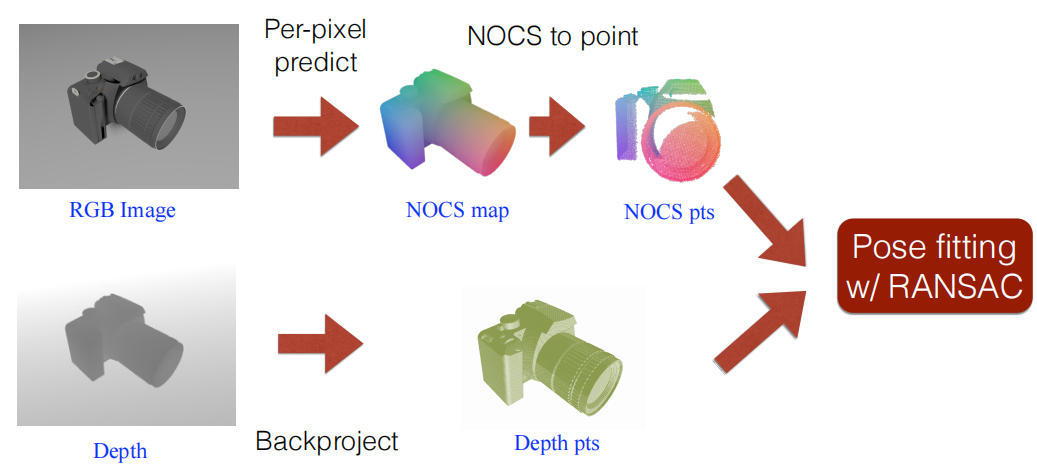
\includegraphics[scale=0.65]{figures/image_nocs_pose.png}
   \caption{From Image to NOCS map to Pose.}
   \label{}
\end{figure}

\subsection{Beyond Object Pose}
human/hand pose extimation.人体可以按照关节活动,并不是刚体.
